\documentclass[a4paper,12pt]{article}
\usepackage{learnpackage}


\newcommand{\mkst}{\makebox[-3pt][r]{\color{blue}\ding{78}}}
\newcommand{\lbf}[1]{\kaishu\textbf{\color{cyan}#1}}
\newcommand{\lsn}[1]{\noindent\textsc{\color{orange} #1.}}
\newcommand{\lunl}[1]{\underline{\hbox to #1{}}}%%  可输入长度的下划线

\setlength{\headheight}{14.9998pt}
\addtolength{\topmargin}{-2.49998pt}

\pgfplotsset{compat=1.18}

%------------------Document----------------------------

\begin{document}

%-------------------------TitlePage------------------------
%\begin{titlepage}
%\end{titlepage}

%-------------------------Content------------------------
\section{功能关系}
\subsection{功}

\lsn{1}功的定义：\lunl{20em}

\lsn{2}功的正负与\(F\)和\(x\)的夹角\(\theta\)的关系:
\vspace*{2cm}

\lsn{3}重力做功：\lunl{20em}

{\noindent\fangsong 如图下图所示，质量为\(m\)的小球从\(B\)点沿着半径为\(R\)的圆形竖直轨道运动到\(A\)点，写出重力做功的表达式。}
\begin{figure}[htbp]
  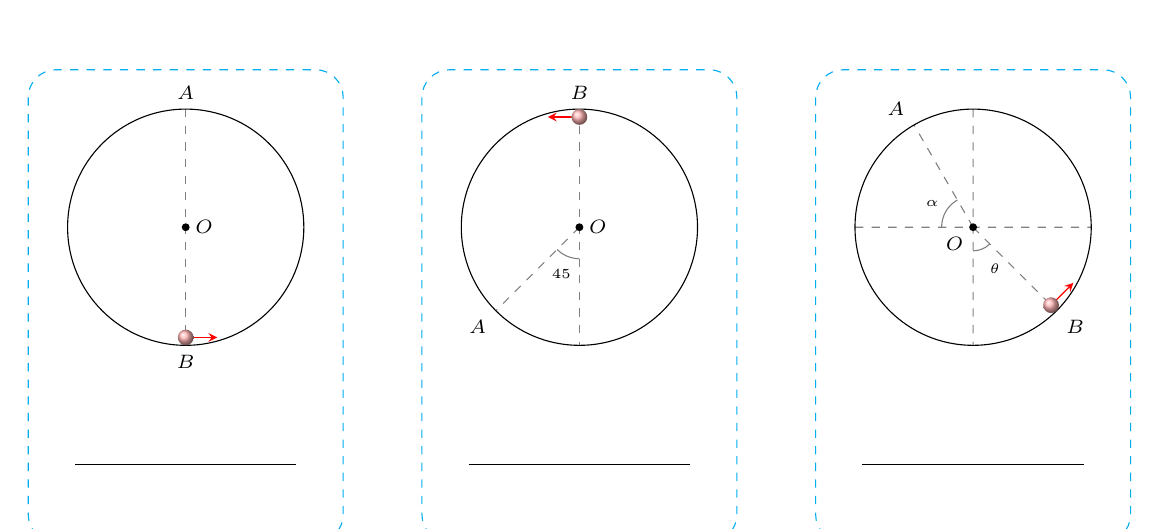
\begin{tikzpicture}
    \begin{scope}
      \draw[dashed,cyan,rounded corners=10] (-2,2) rectangle(2,-4);
      \draw[dashed,gray,font=\scriptsize] (0,1.5)node[above,black]{\(A\)}--(0,-1.5)node[below,black]{\(B\)};
      \draw (0,0) circle(1.5);
      \fill (0,0)node[right,font=\scriptsize]{\(O\)} circle
      (.05);
      \draw[-stealth,red] (0,-1.4)--++(.4,0);
      \shade[ball color=red!30] (0,-1.4) circle(.1);
      \node at(0,-3){\text{\lunl{8em}}};
    \end{scope}
    \begin{scope}[xshift=5cm]
      \draw[dashed,cyan,rounded corners=10] (-2,2) rectangle(2,-4);
      \draw[dashed,gray,font=\scriptsize] (0,1.5)node[above,black]{\(B\)}--(0,-1.5);
      \draw[dashed,gray,font=\scriptsize] (0,0)--(-135:1.5) node[below left,black]{\(A\)};
      \draw[gray] (0,-.4) arc(-90:-135:.4);
      \node[font=\tiny] at(-.25,-.6){\,\qty{45}{\degree}};
      \draw (0,0) circle(1.5);
      \fill (0,0)node[right,font=\scriptsize]{\(O\)} circle
      (.05);
      \draw[-stealth,red] (0,1.4)--++(-.4,0);
      \shade[ball color=red!30] (0,1.4) circle(.1);
      \node at(0,-3){\text{\lunl{8em}}};
    \end{scope}
    \begin{scope}[xshift=10cm]
      \draw[dashed,cyan,rounded corners=10] (-2,2) rectangle(2,-4);
      \draw[dashed,gray,font=\scriptsize] (0,1.5)--(0,-1.5) (-1.5,0)--(1.5,0) (0,0)--(-45:1.5)node[below right,black]{\(B\)} (0,0)--(120:1.5)node[above left,black]{\(A\)};
      \draw[gray] (0,-.3) arc(-90:-45:.3) (120:.4) arc(120:180:.4);
      \node[font=\tiny] at(-62.5:.6){\(\theta\)};
      \node[font=\tiny] at(150:.6){\(\alpha\)};
      \draw (0,0) circle(1.5);
      \fill (0,0)node[below left,font=\scriptsize]{\(O\)} circle(.05);
      \draw[-stealth,red] (-45:1.4)--++(45:0.4);
      \shade[ball color=red!30] (-45:1.4) circle(.1);
      \node at(0,-3){\text{\lunl{8em}}};
    \end{scope}
\end{tikzpicture}

\end{figure}

\lsn{4}摩擦力做功：\lunl{20em}

\begin{figure}[htbp]
  \begin{tikzpicture}[scale=0.95]
    \begin{scope}
      \draw[dashed,cyan,rounded corners=10] (-2,0) rectangle(2,-4);
      \node[font=\tiny] at(0,-.5){\kaishu 给出一个静摩擦力做负功的情景：};
    \end{scope}
    \begin{scope}[xshift=4.2cm]
      \draw[dashed,cyan,rounded corners=10] (-2,0) rectangle(2,-4);
      \node[font=\tiny] at(0,-.5){\kaishu 给出一个静动摩擦力做正功的情景：};
    \end{scope}
    \begin{scope}[xshift=8.4cm]
      \draw[dashed,cyan,rounded corners=10] (-2,0) rectangle(2,-4);
      \node[font=\tiny] at(0,-.5){\kaishu 给出一个滑动摩擦力做负功的情景：：};
    \end{scope}
    \begin{scope}[xshift=12.6cm]
      \draw[dashed,cyan,rounded corners=10] (-2,0) rectangle(2,-4);
      \node[font=\tiny] at(0,-.5){\kaishu 给出一个滑动摩擦力做正功的情景：};
    \end{scope}
  \end{tikzpicture}
\end{figure}

\lsn{5}求变力做功的两种方法:

\begin{figure}[htbp]
  \begin{tikzpicture}
    \begin{scope}
      \draw[dashed,cyan,rounded corners=10] (0,0) rectangle(7,-3);
      \node[font=\tiny] at(.5,-.5){\ding{172}};
    \end{scope}
    \begin{scope}[xshift=8cm]
      \draw[dashed,cyan,rounded corners=10] (0,0) rectangle(7,-3);
      \node[font=\tiny] at(.5,-.5){\ding{173}};
    \end{scope}
  \end{tikzpicture}
\end{figure}

\newpage
\subsection{功率}
\lsn{1}功率的定义（{\kaishu 公式}）：\lunl{10em}

\lsn{2}功率的物理意义：\lunl{20em}

\lsn{3}功率公式的简单推导:
\vspace*{1cm}

\lsn{4}平均功率与瞬时功率的区别：
\vspace*{1cm}


\subsection{机车启动}

{\kaishu 一质量为\(m\)汽车车的额定功率为\(P_0\)，行驶过程中受到的阻力恒为\(f\)，汽车发动机产生的牵引力用\(F\)表示，回答下列问题：}

\lsn{1}以额定功率启动:作出\(v - t\)图像、\(F - t\)图像、\(P - t\)图像，并简要说明原因。
\begin{figure}[htbp]
  \begin{tikzpicture}
    \begin{scope}
      \draw[-latex,blue,font=\scriptsize] (0,0)node[below left]{\(O\)}--(4,0)node[below]{\(t\)};
      \draw[-latex,blue,font=\scriptsize] (0,0)--(0,3)node[left]{\(v\)};
    \end{scope}
    \begin{scope}[xshift=5cm]
      \draw[-latex,blue,font=\scriptsize] (0,0)node[below left]{\(O\)}--(4,0)node[below]{\(t\)};
      \draw[-latex,blue,font=\scriptsize] (0,0)--(0,3)node[left]{\(P\)};
    \end{scope}
    \begin{scope}[xshift=10cm]
      \draw[-latex,blue,font=\scriptsize] (0,0)node[below left]{\(O\)}--(4,0)node[below]{\(t\)};
      \draw[-latex,blue,font=\scriptsize] (0,0)--(0,3)node[left]{\(F\)};
    \end{scope}
  \end{tikzpicture}
\end{figure}
\vspace*{3cm}
  
\lsn{2}以恒定加速度\(a\)启动:作出\(v - t\)图像、\(F - t\)图像、\(P - t\)图像，并简要说明原因。
\begin{figure}[htbp]
  \begin{tikzpicture}
    \begin{scope}
      \draw[-latex,blue,font=\scriptsize] (0,0)node[below left]{\(O\)}--(4,0)node[below]{\(t\)};
      \draw[-latex,blue,font=\scriptsize] (0,0)--(0,3)node[left]{\(v\)};
    \end{scope}
    \begin{scope}[xshift=5cm]
      \draw[-latex,blue,font=\scriptsize] (0,0)node[below left]{\(O\)}--(4,0)node[below]{\(t\)};
      \draw[-latex,blue,font=\scriptsize] (0,0)--(0,3)node[left]{\(P\)};
    \end{scope}
    \begin{scope}[xshift=10cm]
      \draw[-latex,blue,font=\scriptsize] (0,0)node[below left]{\(O\)}--(4,0)node[below]{\(t\)};
      \draw[-latex,blue,font=\scriptsize] (0,0)--(0,3)node[left]{\(F\)};
    \end{scope}
  \end{tikzpicture}
\end{figure}
\newpage

\subsection{势能}
\lsn{1}重力做功的特点：
\vspace*{1cm}

\lsn{2}重力势能的定义：\lunl{20em}
\vspace*{1cm}

{\fangsong 如下所示，质量均匀分布的长为\(3L\) 质量为\(3m\)的铁丝折成不同形状放置在地面上，以地面为零势面，则重力势能为：}
\begin{figure}[htbp]
  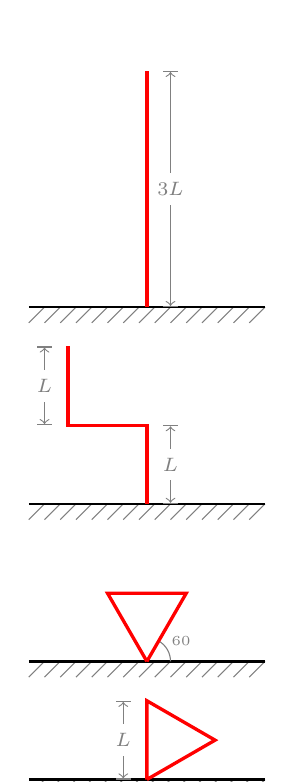
\begin{tikzpicture}
    \begin{scope}
      \foreach \x in{-1.5,-1.3,...,1.3}
      \draw[gray] (\x,-.2)--++(.2,.2);
      \draw[thick] (-1.5,0)--(1.5,0); 
      \draw[|<->|,gray,thin,font=\scriptsize] (.3,0)--node[fill=white]{\(3L\)}(.3,3);
      \draw[very thick,red] (0,0)--(0,3);
    \end{scope}
    \begin{scope}[yshift=-2.5cm]
      \foreach \x in{-1.5,-1.3,...,1.3}
      \draw[gray] (\x,-.2)--++(.2,.2);
      \draw[thick] (-1.5,0)--(1.5,0);
      \draw[very thick,red] (0,0)--(0,1)--(-1,1)--(-1,2);
      \draw[|<->|,gray,thin,font=\scriptsize] (.3,0)--node[fill=white]{\(L\)}(.3,1);
      \draw[|<->|,gray,thin,font=\scriptsize] (-1.3,1)--node[fill=white]{\(L\)}(-1.3,2);
    \end{scope}
    \begin{scope}[yshift=-4.5cm]
      \foreach \x in{-1.5,-1.3,...,1.3}
      \draw[gray] (\x,-.2)--++(.2,.2);
      \draw[thick] (-1.5,0)--(1.5,0); 
      \draw[gray] (.3,0) arc(0:60:.3)node[right,font=\tiny]{\,\qty{60}{\degree}};
      \draw[very thick,red] (0,0)--++(60:1)--++(-1,0)--(0,0);
    \end{scope}
    \begin{scope}[yshift=-6cm]
      \foreach \x in{-1.5,-1.3,...,1.3}
      \draw[gray] (\x,-.2)--++(.2,.2);
      \draw[thick] (-1.5,0)--(1.5,0); 
      \draw[|<->|,gray,thin,font=\scriptsize] (-.3,0)--node[fill=white]{\(L\)}(-.3,1);
      \draw[very thick,red] (0,0)--(0,1)--++(-30:1)--(0,0);
    \end{scope}
  \end{tikzpicture}
\end{figure}

\lsn{3}重力做功与重力势能变化量的关系（{\kaishu 写出公式并给出推导过程}）：
\vspace*{3cm}

\lsn{4}弹簧弹性势能（{\kaishu 公式}）：\lunl{10em}

{\fangsong 将一劲度系数为\(k\)的弹簧拉伸，其形变量为\(x\)，求这一过程中确弹簧弹力所做的功？}

\newpage
\subsection{动能定理}
\lsn{1}动能的定义（{\kaishu 公式}）：\lunl{10em}

\lsn{2}动能定理内容（{\kaishu 文字}）：
\vspace*{1cm}

\lsn{3}动能定理表达式：\lunl{20em}

\lsn{4}动能定理的简单推导：

\begin{tikzpicture}
  \draw[thick] (0,0)--(5.2,0);
  \draw[fill=orange!50] (.2,0) rectangle(.6,.4);
  \draw[->,font=\scriptsize] (.2,.5)--node[above]{\(v_1\)}(.6,.5);
  \node[font=\scriptsize] at(.4,.2){\(m\)};
  \draw[draw=gray,fill=orange!30] (4.2,0) rectangle(4.6,.4);
  \draw[->,font=\scriptsize] (4.2,.5)--node[above]{\(v_2\)}(4.6,.5);
  \draw[->,font=\scriptsize] (.6,.2)--++(.5,0)node[right]{\(F\)};
  \draw[|->|] (.6,-.2)--node[below]{\(x\)}(4.6,-.2);
  \node[font=\tiny] at(2.5,1){{\kaishu 地面光滑}};
\end{tikzpicture}

\vspace*{1cm}
\lsn{5}动能定理的应用流程：
\vspace*{4cm}
\subsection{动能定理与竖直圆周运动}
\lsn{1}如下图所示，长为\(l\)的轻绳系一质量为\(m\)的小球，轻绳与竖直方向的夹角为\(\theta\)，小球从\(A\)点静止释放运动到最低点\(B\)，求小球在\(A\)点时绳上的拉力\(T_A\)，小球在\(B\)点时绳上的拉力\(T_B\)，小球在\(B\)点的速度\(v_B\)。
\begin{figure}[htbp]
  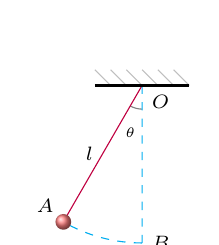
\begin{tikzpicture}
  \draw[gray] (0,-.3) arc(-90:-120:.3);
  \draw[purple,font=\scriptsize] (0,0)--node[left,black]{\(l\)}(-120:2);
  \node[font=\tiny]  at(-.15,-.6){\(\theta\)};
  \draw[dashed,cyan,font=\scriptsize] (-90:2) arc(-90:-120:2) (0,0)node[below right,black]{\(O\)}--(0,-2)node[right,black]{\(B\)};
  \shade[ball color=red!50,font=\scriptsize] (-120:2)node[above left]{\(A\)} circle(.1);
  \foreach \x in{-.6,-.4,...,.6}
  \draw[gray!50] (\x,.2)--++(.2,-.2);
  \draw[thick] (-.6,0)--(.6,0);
\end{tikzpicture}
\end{figure}

\newpage
\lsn{2}如下图所示，质量均为\(m\)的小球从\(A\)点以初速度\(v_0\) 沿半径为\(R\)的光滑竖直轨道（管道）向上运动，且匀{\kaishu\color{red}\lud{恰好}}运动到\(B\)点，求初速度\(v_0\)。
\begin{figure}[htbp]
  \begin{tikzpicture}[scale=.91]
    \begin{scope}[yshift=5.5cm]
      \draw[dashed,cyan,rounded corners=10] (-2,2) rectangle(2,-3);
      \draw[dashed,gray,font=\scriptsize] (0,1.5)--(0,-1.5)node[below left,black]{\(A\)} (-1.5,0)--(1.5,0)node[right,black]{\(B\)};
      \draw (0,0) circle(1.5);
      \fill (0,0)node[below left,font=\scriptsize]{\(O\)} circle(.05);
      \draw[-stealth,red] (-90:1.4)--++(0:0.4);
      \shade[ball color=red!30] (-90:1.4) circle(.1);
    \end{scope}
    \begin{scope}[xshift=0cm]
      \draw[dashed,cyan,rounded corners=10] (-2,2) rectangle(2,-3);
      \draw[dashed,gray,font=\scriptsize] (0,1.5)node[above,black]{\(B\)}--(0,-1.5)node[below left,black]{\(A\)} (-1.5,0)--(1.5,0) (45:0);
      \draw (0,0) circle(1.5);
      \fill (0,0)node[below left,font=\scriptsize]{\(O\)} circle(.05);
      \draw[-stealth,red] (-90:1.4)--++(0:0.4);
      \shade[ball color=red!30] (-90:1.4) circle(.1);
    \end{scope}
    \begin{scope}[yshift=-5.5cm]
      \draw[dashed,cyan,rounded corners=10] (-2,2) rectangle(2,-3);
      \draw[dashed,gray,font=\scriptsize] (0,1.5)--(0,-1.5)node[below left,black]{\(A\)} (-1.5,0)--(1.5,0) (0,0)--(45:1.5)node[above right,black]{\(B\)};
      \draw[gray] (.2,0) arc(0:45:.2);
      \node[font=\tiny] at(.5,.15){\(\theta\)};
      \draw (0,0) circle(1.5);
      \fill (0,0)node[below left,font=\scriptsize]{\(O\)} circle(.05);
      \draw[-stealth,red] (-90:1.4)--++(0:0.4);
      \shade[ball color=red!30] (-90:1.4) circle(.1);
    \end{scope}
    \begin{scope}[yshift=-11cm]
      \draw[dashed,cyan,rounded corners=10] (-2,2) rectangle(2,-3);
      \draw[dashed,gray,font=\scriptsize] (0,1.5)node[above,black]{\(B\)}--(0,-1.5)node[below left,black]{\(A\)} (-1.5,0)--(1.5,0);
      \draw (0,0) circle(1.5) (0,0) circle(1.3);
      \fill (0,0)node[below left,font=\scriptsize]{\(O\)} circle(.05);
      \draw[-stealth,red] (-90:1.4)--++(0:0.4);
      \shade[ball color=red!30] (-90:1.4) circle(.1);
      \node[font=\tiny] at(0,-2.2){\kaishu 管道内径可忽略};
    \end{scope}
  \end{tikzpicture}
\end{figure}


\newpage
\subsection{机械能守恒定律}
\lsn{1}机械能的定义：
\vspace*{1cm}

\lsn{2}机械能与内能的区别：
\vspace*{1cm}

\lsn{3}机械能守恒定律的内容：
\vspace*{2cm}

\lsn{4}如何判断机械能是否守恒：
\vspace*{1cm}

\lsn{5}机械能守恒定律应用步骤：
\vspace*{3cm}

\lsn{6}实例应用：如下图所示，可绕\(O\)点自由转运的长为\(2l\)的轻杆在中点和末端分别固定质量为\(2m\) 和\(m\)的小球\(A\)和\(B\)，杆在水平位置静止释放，求杆摆到坚直位置时\(A\)、\(B\)两球的速度\(v_1\)、\(v_2\)。
\begin{figure}[htbp]
  \begin{tikzpicture}
    \draw[cyan,dashed] (0,0)--(0,-3) arc(-90:0:3) (0,-1.5) arc(-90:0:1.5);
    \draw[thick,font=\scriptsize] (0,0)node[above]{\(O\)}--(3,0);
    \shade[ball color=red!50,font=\scriptsize] (1.5,0)node[above]{\(A\)} circle(.1);
    \shade[ball color=red!50,font=\scriptsize] (3,0)node[above]{\(B\)} circle(.1);
  \end{tikzpicture}
\end{figure}
\end{document}
